%%%%%%%%%%%%%%%%%%%%%%%%%%%%%%%%%%%%%%%%%
% Wilson Resume/CV
% XeLaTeX Template
% Version 1.0 (22/1/2015)
%
% This template has been downloaded from:
% http://www.LaTeXTemplates.com
%
% Original author:
% Howard Wilson (https://github.com/watsonbox/cv_template_2004) with
% extensive modifications by Vel (vel@latextemplates.com)
%
% License:
% CC BY-NC-SA 3.0 (http://creativecommons.org/licenses/by-nc-sa/3.0/)
%
%%%%%%%%%%%%%%%%%%%%%%%%%%%%%%%%%%%%%%%%%

%----------------------------------------------------------------------------------------
%	PACKAGES AND OTHER DOCUMENT CONFIGURATIONS
%----------------------------------------------------------------------------------------
\documentclass[11pt]{article} % Default font size
\usepackage{graphicx}
\usepackage{enumitem}
\graphicspath{ {images/} }
\thispagestyle{empty}
% * <spencer.tengz@gmail.com> 2018-04-27T13:12:11.200Z:
%
% ^.
%%%%%%%%%%%%%%%%%%%%%%%%%%%%%%%%%%%%%%%%%
% Wilson Resume/CV
% Structure Specification File
% Version 1.0 (22/1/2015)
%
% This file has been downloaded from:
% http://www.LaTeXTemplates.com
%
% License:
% CC BY-NC-SA 3.0 (http://creativecommons.org/licenses/by-nc-sa/3.0/)
%
%%%%%%%%%%%%%%%%%%%%%%%%%%%%%%%%%%%%%%%%%

%----------------------------------------------------------------------------------------
%	PACKAGES AND OTHER DOCUMENT CONFIGURATIONS
%----------------------------------------------------------------------------------------

\usepackage[a4paper, hmargin=10mm, vmargin=15mm, top=10mm]{geometry} % Use A4 paper and set margins

\usepackage{fancyhdr} % Customize the header and footer

\usepackage{lastpage} % Required for calculating the number of pages in the document

\usepackage{hyperref} % Colors for links, text and headings

\setcounter{secnumdepth}{0} % Suppress section numbering

%\usepackage[proportional,scaled=1.064]{erewhon} % Use the Erewhon font
%\usepackage[erewhon,vvarbb,bigdelims]{newtxmath} % Use the Erewhon font
\usepackage[utf8]{inputenc} % Required for inputting international characters
\usepackage[T1]{fontenc} % Output font encoding for international characters

\usepackage{fontspec} % Required for specification of custom fonts
\setmainfont[Path = ./fonts/,
Extension = .otf,
BoldFont = Erewhon-Bold,
ItalicFont = Erewhon-Italic,
BoldItalicFont = Erewhon-BoldItalic,
SmallCapsFeatures = {Letters = SmallCaps}
]{Erewhon-Regular}

\usepackage{color} % Required for custom colors
\definecolor{slateblue}{rgb}{0.17,0.22,0.34}

\usepackage{sectsty} % Allows customization of titles
\sectionfont{\color{slateblue}} % Color section titles

\fancypagestyle{plain}{\fancyhf{}\cfoot{\thepage\ of \pageref{LastPage}}} % Define a custom page style
\pagestyle{plain} % Use the custom page style through the document
\renewcommand{\headrulewidth}{0pt} % Disable the default header rule
\renewcommand{\footrulewidth}{0pt} % Disable the default footer rule

\setlength\parindent{0pt} % Stop paragraph indentation

% Non-indenting itemize
\newenvironment{itemize-noindent}
{\setlength{\leftmargini}{0em}\begin{itemize}}
{\end{itemize}}

% Text width for tabbing environments
\newlength{\smallertextwidth}
\setlength{\smallertextwidth}{\textwidth}
\addtolength{\smallertextwidth}{-2cm}

\newcommand{\sqbullet}{~\vrule height 0.1ex width .8ex depth -.2ex} % Custom square bullet point definition

%----------------------------------------------------------------------------------------
%	MAIN HEADER COMMAND
%----------------------------------------------------------------------------------------

\renewcommand{\title}[1]{
{{\color{slateblue}\Huge\textbf{%
#1
}}}
}
%----------------------------------------------------------------------------------------
%	JOB COMMAND
%----------------------------------------------------------------------------------------

\newcommand{\job}[6]{
\begin{tabbing}
\hspace{2cm} \= \kill
\textbf{#1} \> \href{#4}{#3} \\
\textbf{#2} \>\+ \textit{#5} \\
\begin{minipage}{\smallertextwidth}
\vspace{2mm}
#6
\end{minipage}
\end{tabbing}
\vspace{1mm}
}

%----------------------------------------------------------------------------------------
%	SKILL GROUP COMMAND
%----------------------------------------------------------------------------------------

\newcommand{\skillgroup}[2]{
\begin{tabbing}
\hspace{5mm} \= \kill
\sqbullet \>\+ \textbf{#1} \\
\begin{minipage}{\smallertextwidth}
\vspace{1mm}
#2
\end{minipage}
\end{tabbing}
}

%----------------------------------------------------------------------------------------
%	INTERESTS GROUP COMMAND
%-----------------------------------------------------------------------------------------

\newcommand{\interestsgroup}[1]{
\begin{tabbing}
\hspace{5mm} \= \kill
#1
\end{tabbing}
\vspace{-10mm}
}

\newcommand{\interest}[1]{\sqbullet \> \textbf{#1}\\[3pt]} % Define a custom command for individual interests

%----------------------------------------------------------------------------------------
%	TABBED BLOCK COMMAND
%----------------------------------------------------------------------------------------

\newcommand{\tabbedblock}[1]{
\begin{tabbing}
\hspace{2cm} \= \hspace{4cm} \= \kill
#1
\end{tabbing}
} % Include the file specifying document layout

%----------------------------------------------------------------------------------------

\begin{document}

{\fontfamily{lmss}\selectfont


%----------------------------------------------------------------------------------------
%	NAME 
%----------------------------------------------------------------------------------------

\hspace{-1.2em}\title{ Spencer Teng } % Print the main header

\noindent\begin{minipage}[t]{0.8\textwidth}
\vspace{1em}
%\textbf{Machine Learning Engineer} \\

Versatile data scientist with multi-year hand-on experience building AI-powered applications such
as recommendation, medical image analysis, and chatbot.
Goal-oriented, autonomous,
and strong problem-solving engineer. 
%Looking forward to a new journey in applied machine learning fields.
%----------------------------------------------------------------------------------------
%	Certificate
%----------------------------------------------------------------------------------------

% \section{Certificates}
% \begin{itemize}
% \item{Deep Learning Specialization - Coursera (License DCVAEL4SGCRC)}
% \end{itemize}

%----------------------------------------------------------------------------------------
%	SKILLS SECTION
%----------------------------------------------------------------------------------------
\section{Skills}

Python, Machine Learning, Deep learning, Keras, TensorFlow, Scikit-learn, Pandas, Plotly, Django REST, Git, Docker, Linux/Unix, Scrum


%----------------------------------------------------------------------------------------
%	PERSONAL PROFILE AND CONTACT INFORMATION
%----------------------------------------------------------------------------------------
\end{minipage}\hspace{1mm}
\begin{minipage}[t]{0.22\textwidth}
\raisebox{\dimexpr-\height+\ht\strutbox}{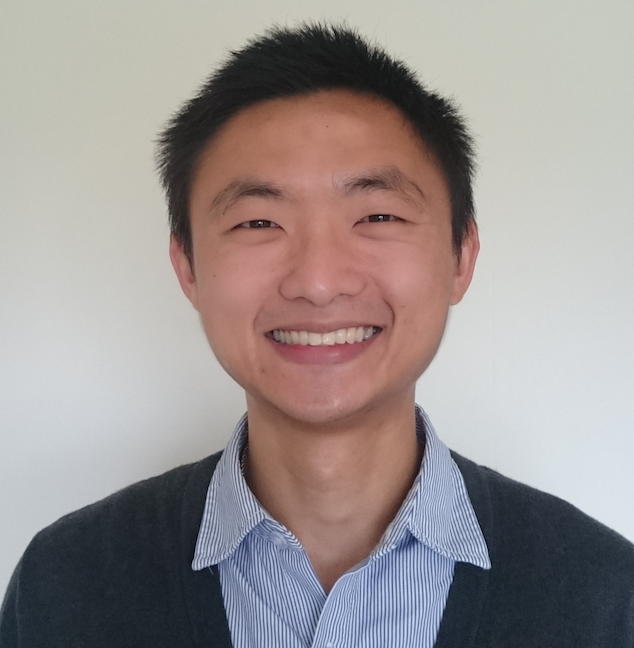
\includegraphics[height=0.8\textwidth, width=0.8\textwidth]{profile.png}}



\begin{tabbing} % Enables tabbing
%\hspace{2cm} \= \hspace{2cm} \= \kill % Spacing within the block
%\textbf{Contact Info} \\ 

spencer.tengz@gmail.com \\ % Email address
linkedin.com/in/spencerimp/ \\ % LinkedIn
+45 50 12 28 50 \\ % Mobile phone
\end{tabbing}
\end{minipage}

%----------------------------------------------------------------------------------------
%	Experience
%----------------------------------------------------------------------------------------

\section{Experience}
\job
{Oct 2022 }{Present}
{\textbf{Machine Learning Engineer}}
{}
{Pandora, CPH, Denmark}
{
	
	Developing personalized recommendation pipelines
	\begin{itemize}[itemsep=0pt]
		\item Developing MLOps for recommendation pipelines such as  training automation, monitoring, etc.
		%\item Tech stack: TensorFlow, Django Rest, Celery, Java Spring Boot, Elastic Stack, etc.
	\end{itemize}
}
\job
{Oct 2018 }{Sep 2021}
{\textbf{Machine Learning Engineer}}
{}
{Data Science Lab, Nordea Bank, CPH, Denmark}
{
 
    Developed Innova, Nordea in-house chatbot using Natural Language Processing techniques.
    \begin{itemize}[itemsep=0pt]
    	\item  Developed chatbot REST APIs to answer customer questions and perform banking actions..
    	\item  Automated machine learning retraining and deployment in production.
    	\item  Introduced model inference optimization to reduce ML API latency by 30\%.
    	%\item Tech stack: TensorFlow, Django Rest, Celery, Java Spring Boot, Elastic Stack, etc.
    \end{itemize}
}

\job
{Aug 2017 }{Jun 2018}
{\textbf{Technical Co-founder}}
{}
{GUTXY, Frederiksberg, Denmark}
{
%	Developed bioinformatics pipeline and webapps to analyze gut bacteria and produce a wellness report.\\ 
%	InnoFounder incubator program in 2018 (acceptance rate: 13/102).
	\begin{itemize}[itemsep=0pt]
		\item Developed a bioinformatics product that provides a report to improve customers’ gut health.
		\item InnoFounder incubator program in 2018 (acceptance rate: 13/102).
		%\item Tech stack: Scikit-learn, Django Rest, Qiime2, Matplotlib, AWS EC2, S3, ElasticBeanstalk, etc.
	\end{itemize}
}

\job
{Mar 2017 }{Sep 2021}
{\textbf{Machine Learning Engineer Freelancer}}
{}
{Upwork}
{
%	Top-rated machine learning engineer using mainly Python, Keras, TensorFlow, and OpenCV.\\
%	Projects include object detection, image recognition/segmentation, backend API development.
	Top-rated freelancer specialized in deep learning and computer vision systems.
		\begin{itemize}[itemsep=0pt]
			\item Design and implement production-grade REST APIs for object detection, image segmentation, etc.
			%\item Tech stack: Keras, TensorFlow, OpenCV, Scikit-learn, Django Rest, Docker, AWS EC2, S3, etc.
		\end{itemize}
}

%------------------------------------------------

\job
{Feb 2016 }{Feb 2017}
{\textbf{Research Assistant}}
{}
{Biomediq, CPH, Denmark}
{
%	Developed deep convolutional neural networks for brain MRI segmentation with Python and Keras.\\
%	Published a book chapter in deep learning for medical image analysis.
		\begin{itemize}[itemsep=0pt]
%			\item Developed deep neural network based MRI segmentation pipeline and achieved the state-of-the-art.
			\item Published a book chapter about deep neural net for brain MRI segmentation and analysis.
		\end{itemize}
}

\job
{Aug 2011 }{Aug 2014}
{\textbf{Research Assistant}}
{}
{Music AI Lab, Academic Sinica, Taipei, Taiwan}
{
%	Developed context-aware music recommendation for Android phones with SVM and collaborative filtering.\\
%	Published two papers in international conference and journal.
		\begin{itemize}[itemsep=0pt]
			\item Developed context-aware music recommendation app from data collection to prototyping for HTC.
			\item Published papers in conference and journal about recommendation and user behavior analysis.
		\end{itemize}	
}
%----------------------------------------------------------------------------------------
%	EDUCATION SECTION
%----------------------------------------------------------------------------------------
\section{Education}
\tabbedblock{
\bf{2014-2016} \> M.Sc. Computer Science - University of Copenhagen \\
\>\+Master Thesis: Automated brain MRI segmentation with deep neural networks. \\ 
}
% %------------------------------------------------
% \tabbedblock{
% \bf{2006-2010} \> B.Sc. Computer Science - \textbf{National Taiwan Ocean University,} \\\>\+Keelung, Taiwan
% }

% %----------------------------------------------------------------------------------------
% %	INTERESTS SECTION
% %----------------------------------------------------------------------------------------

% \section{Interests \& Learning}
% Tennis, Cycling, Danish (modul 3)

\end{document}